\chapter[Sprint 1]{Study and Implementation of Sprint 1: Authentication \& Landing Page}

\section{Introduction}
Sprint 1 focuses on developing the authentication system and landing page using NextAuth.js and Prisma ORM. This sprint establishes essential user management capabilities and creates an intuitive entry point for the application, building upon the foundation from previous iterations.

\section{Sprint Planning}

\subsection{Objectives}
\begin{itemize}
    \item Implement secure OAuth authentication (Google, GitHub)
    \item Develop cross-device session management
    \item Create responsive landing page
\end{itemize}
\subsection{Backlog Items}


\begin{table}[H]
    \centering
    \begin{tabular}{|c|l|c|p{8cm}|c|}
    \hline
    \textbf{ID} & \textbf{Feature} & \textbf{Sub-ID} & \textbf{User Story} & \textbf{Priority} \\
    \hline
    1 & Authentication & 1.1 & As a user; I want to authenticate using my Google account. & M \\
    \hline
    1  & Authentication & 1.2 & As a user; I want to authenticate using my GitHub account. & M \\
    \hline
    1  & Authentication & 1.3 & As a user; I want to stay authenticated across multiple devices. & S \\
    \hline
    1  & Authentication & 1.4 & As a user; I want to log out from my account. & M \\
    \hline
    2 & Explore Landing Page & 2.1 & As a user; I want to explore the landing page so that I can understand the platform's features and benefits. & M \\
    \hline
    \end{tabular}
    \caption{User Stories Requirements Table}
    \label{tab:user_stories}
    \end{table}
\section{System Analysis}

\subsection{Use Case Overview}
\begin{figure}[H]
    \centering
    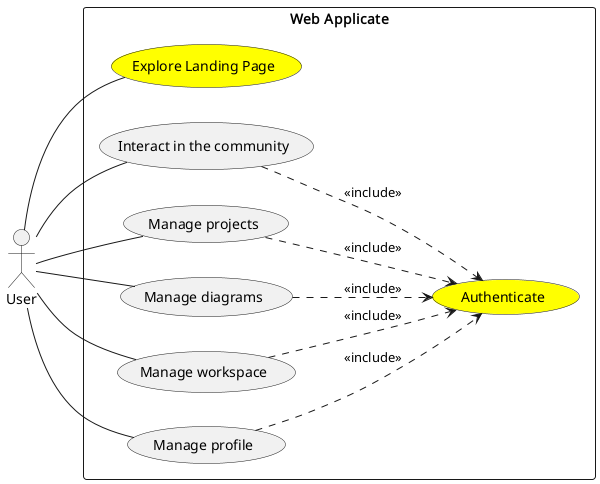
\includegraphics[width=0.8\textwidth]{conception/SprintII/use_case_diagrams/use_case_diagram_of_SprintII.png}
    \caption{Sprint 1 Use Case Diagram}
    \label{fig:usecase_sprint2}
\end{figure}
\newpage
\subsection{Authentication Use Cases}
\begin{figure}[H]
    \centering
    \includegraphics[width=0.8\textwidth]{conception/SprintII/use_case_diagrams/refined_use_case_feature_auth.png}
    \caption{Refined Authentication Use Case}
    \label{fig:refined_auth_usecase}
\end{figure}

\subsubsection{Core Authentication Scenarios}

\textbf{OAuth Sign-In Process:}
\begin{enumerate}
    \item User clicks OAuth provider button (Google/GitHub)
    \item System redirects to provider's authorization page
    \item User authorizes application access
    \item Provider returns authorization code
    \item System validates and creates user session
    \item User is redirected to dashboard
\end{enumerate}

\textbf{Cross-Device Authentication:}
Session persistence is maintained through secure tokens allowing users to access the application across multiple devices without re-authentication, with automatic session validation and expiration handling.

\textbf{Secure Sign-Out:}
Session termination involves token invalidation, cookie clearing, and secure redirection to the landing page.

\section{Sequence Diagrams}

\begin{figure}[H]
    \centering
    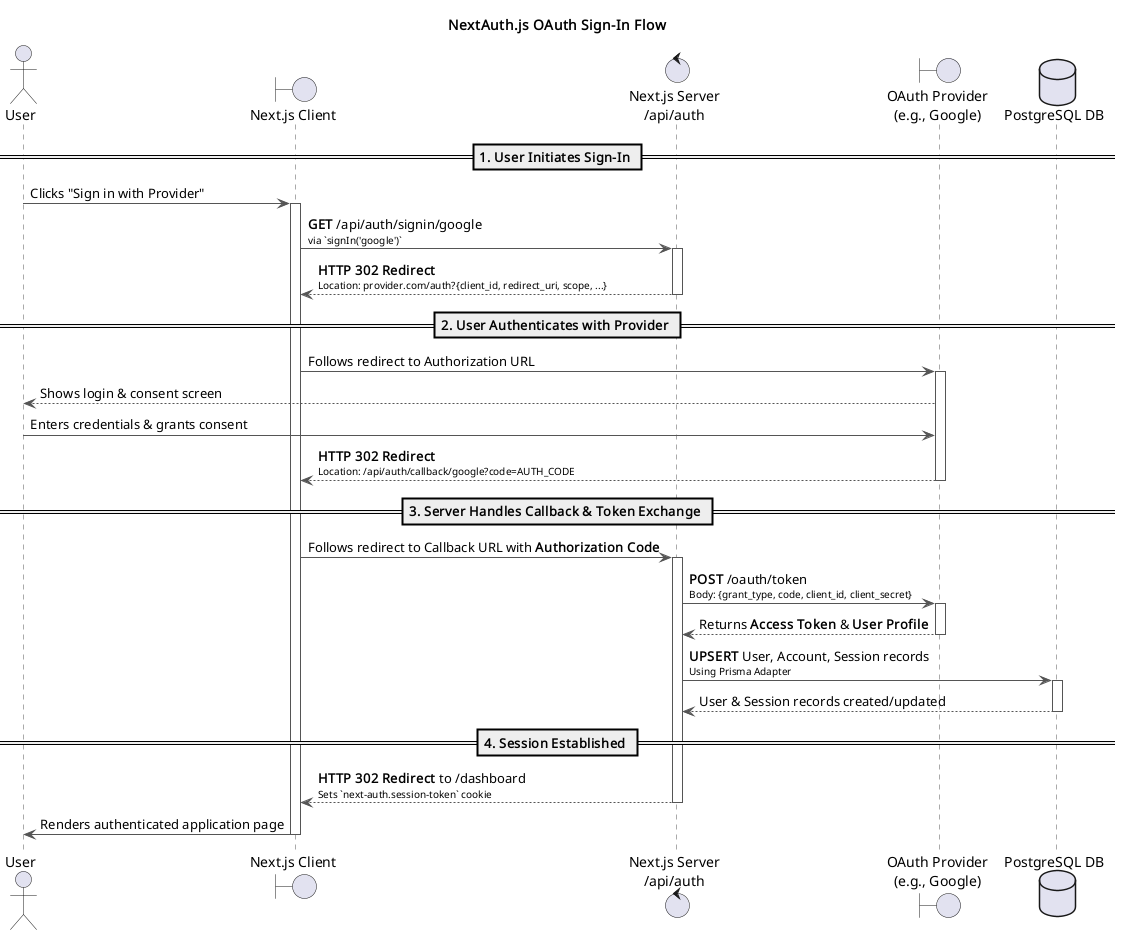
\includegraphics[width=1\textwidth]{conception/SprintII/sequence_diagrams/sequence_authentication_1_1_AuthenticateUsingGoogleAccount.png}
    \caption{OAuth Authentication Sequence}
    \label{fig:seq_google_auth}
\end{figure}


\section{Implementation Results}

\subsection{Landing Page}
\begin{figure}[H]
    \centering
    \includegraphics[width=1.0\textwidth]{screenshots/landing.png}
    \caption{Responsive Landing Page}
    \label{fig:landing_page}
\end{figure}

Modern design featuring clear value proposition, feature highlights, and prominent call-to-action elements optimized for user engagement and conversion.

\subsection{Authentication Interface}
\begin{figure}[H]
    \centering
    \includegraphics[width=0.8\textwidth]{screenshots/signin.png}
    \caption{OAuth Sign-In Interface}
    \label{fig:signin_page}
\end{figure}

Clean, user-friendly authentication interface supporting multiple OAuth providers with consistent branding and accessibility standards.

\section{Sprint Retrospective}

\textbf{Achievements:}
\begin{itemize}
    \item Successful OAuth integration with Google and GitHub
    \item Robust cross-device session management
    \item Responsive landing page with high conversion potential
    \item Secure authentication flow with proper error handling
\end{itemize}

\textbf{Challenges Resolved:}
\begin{itemize}
    \item OAuth configuration complexities across environments
    \item Session persistence optimization
    \item Cross-browser compatibility testing
\end{itemize}

\section{Conclusion}

Sprint 1 successfully established the authentication infrastructure and user entry point. The implementation of NextAuth.js with OAuth providers and Prisma database management provides a secure, scalable foundation for user management. The responsive landing page effectively communicates value while guiding user engagement. These achievements create a solid foundation for subsequent development phases, with robust security and optimal user experience.